%----------------------------------------------------------------------------------------
%	PACKAGES AND OTHER DOCUMENT CONFIGURATIONS
%----------------------------------------------------------------------------------------
\documentclass{article}
\PassOptionsToPackage{latin9}{inputenc} % latin9 (ISO-8859-9) = latin1+"Euro sign"
\usepackage{inputenc}
 
 %------------------------------------------------

\usepackage{fancyvrb}

%\PassOptionsToPackage{ngerman,american}{babel}  % Change this to your language(s)
% Spanish languages need extra options in order to work with this template
%\PassOptionsToPackage{spanish,es-lcroman}{babel}
\usepackage[english]{babel}

\usepackage{listings}
\usepackage{amsmath,bm}
\usepackage{fancyhdr} % Required for custom headers
\usepackage{lastpage} % Required to determine the last page for the footer
\usepackage{extramarks} % Required for headers and footers
% \usepackage[usenames,dvipsnames]{color} % Required for custom colors
\usepackage{graphicx} % Required to insert images
% \usepackage{listings} % Required for insertion of code
\usepackage{courier} % Required for the courier font
\usepackage{lipsum} % Used for inserting dummy 'Lorem ipsum' text into the template
\usepackage{url}

%------------------------------------------------			

\PassOptionsToPackage{square,numbers}{natbib}
 \usepackage{natbib}
 
 %------------------------------------------------

\PassOptionsToPackage{fleqn}{amsmath,amssymb} % Math environments and more by the AMS 
 \usepackage{amsmath}
 
 %------------------------------------------------

\PassOptionsToPackage{T1}{fontenc} % T2A for cyrillics
\usepackage{fontenc}

%------------------------------------------------

\usepackage{xspace} % To get the spacing after macros right

%------------------------------------------------

\usepackage{mparhack} % To get marginpar right

%------------------------------------------------

\usepackage{fixltx2e} % Fixes some LaTeX stuff 

%------------------------------------------------

\PassOptionsToPackage{smaller}{acronym} % Include printonlyused in the first bracket to only show 
% acronyms used in the text
\usepackage{acronym} % nice macros for handling all acronyms in the thesis

%------------------------------------------------

%\renewcommand*{\acsfont}[1]{\textssc{#1}} % For MinionPro
% \renewcommand{\bflabel}[1]{{#1}\hfill} % Fix the list of acronyms

%------------------------------------------------

\PassOptionsToPackage{pdftex}{graphicx}
\usepackage{graphicx} 

%----------------------------------------------------------------------------------------
%	FLOATS: TABLES, FIGURES AND CAPTIONS SETUP
%----------------------------------------------------------------------------------------
\usepackage{booktabs}
\usepackage{tabularx} % Better tables
\setlength{\extrarowheight}{3pt} % Increase table row height
\newcommand{\tableheadline}[1]{\multicolumn{1}{c}{\spacedlowsmallcaps{#1}}}
\newcommand{\myfloatalign}{\centering} % To be used with each float for alignment
\usepackage{caption}
\captionsetup{format=hang,font=small}
\usepackage{subfig}  
\usepackage{color}


\definecolor{MyDarkGreen}{rgb}{0.0,0.4,0.0} % This is the color used for comments
\definecolor{Purple}{rgb}{0.75, 0.0, 1.0}
\definecolor{Blue}{rgb}{0.01, 0.28, 1.0}

\lstloadlanguages{Python} % Load Perl syntax for listings, for a list of other languages supported 
% see: ftp://ftp.tex.ac.uk/tex-archive/macros/latex/contrib/listings/listings.pdf
\lstset{language=Python, % Use Perl in this example
        frame=single, % Single frame around code
        basicstyle=\small\ttfamily, % Use small true type font
        keywordstyle=[1]\color{Blue}\bf, % Perl functions bold and blue
        keywordstyle=[2]\color{Purple}, % Perl function arguments purple
        keywordstyle=[3]\color{Blue}\underbar, % Custom functions underlined and blue
        identifierstyle=, % Nothing special about identifiers                                       
        commentstyle=\usefont{T1}{pcr}{m}{sl}\color{MyDarkGreen}\small, 
        stringstyle=\color{Purple}, % Strings are purple
        showstringspaces=false, % Don't put marks in string spaces
        tabsize=5, % 5 spaces per tab
        %
        % Put standard Perl functions not included in the default language here
        morekeywords={rand},
        %
        % Put Perl function parameters here
        morekeywords=[2]{on, off, interp},
        %
        % Put user defined functions here
        morekeywords=[3]{test},
       	%
        morecomment=[l][\color{Blue}]{...}, % Line continuation (...) like blue comment
        numbers=left, % Line numbers on left
        firstnumber=1, % Line numbers start with line 1
        numberstyle=\tiny\color{Blue}, % Line numbers are blue and small
        stepnumber=5 % Line numbers go in steps of 5
}

% Creates a new command to include a perl script, the first parameter is the filename of the script 
% (without .pl), the second parameter is the caption
\newcommand{\myscript}[2]{
\begin{itemize}
\item[]\lstinputlisting[caption=#2,label=#1]{#1.pl}
\end{itemize}
}


%----------------------------------------------------------------------------------------
%	track changes in the file
%   http://mirror.unl.edu/ctan/macros/latex/contrib/changes/changes.english.pdf
%----------------------------------------------------------------------------------------

\usepackage[deletedmarkup=xout]{changes}
%\newcommand{\todo}[1]{\textcolor{red}{{\textbf{To-Do:} #1}}}
\definecolor{darkgreen}{RGB}{0,100,0}
\definechangesauthor[name={Marten J{\"{a}}ger}, color={darkgreen}]{MJ}


% Margins
\topmargin=-0.45in
\evensidemargin=0in
\oddsidemargin=0in
\textwidth=6.5in
\textheight=9.0in
\headsep=0.25in

\linespread{1.1} % Line spacing

% Set up the header and footer
\pagestyle{fancy}
\lhead{\hmwkAuthorName} % Top left header
\chead{\hmwkClass\ (\hmwkClassInstructor\ \hmwkClassTime): \hmwkTitle} % Top center head
\rhead{\firstxmark} % Top right header
\lfoot{\lastxmark} % Bottom left footer
\cfoot{} % Bottom center footer
\rfoot{Page\ \thepage\ of\ \protect\pageref{LastPage}} % Bottom right footer
\renewcommand\headrulewidth{0.4pt} % Size of the header rule
\renewcommand\footrulewidth{0.4pt} % Size of the footer rule

\setlength\parindent{0pt} % Removes all indentation from paragraphs

%----------------------------------------------------------------------------------------
%	CODE INCLUSION CONFIGURATION
%----------------------------------------------------------------------------------------


%----------------------------------------------------------------------------------------
%	DOCUMENT STRUCTURE COMMANDS
%	Skip this unless you know what you're doing
%----------------------------------------------------------------------------------------

% Header and footer for when a page split occurs within a problem environment
\newcommand{\enterProblemHeader}[1]{
\nobreak\extramarks{#1}{#1 continued on next page\ldots}\nobreak
\nobreak\extramarks{#1 (continued)}{#1 continued on next page\ldots}\nobreak
}

% Header and footer for when a page split occurs between problem environments
\newcommand{\exitProblemHeader}[1]{
\nobreak\extramarks{#1 (continued)}{#1 continued on next page\ldots}\nobreak
\nobreak\extramarks{#1}{}\nobreak
}

\setcounter{secnumdepth}{0} % Removes default section numbers
\newcounter{homeworkProblemCounter} % Creates a counter to keep track of the number of problems

\newcommand{\homeworkProblemName}{}
\newenvironment{homeworkProblem}[1][Problem \arabic{homeworkProblemCounter}]{ %
\stepcounter{homeworkProblemCounter} % Increase counter for number of problems
\renewcommand{\homeworkProblemName}{#1} % Assign \homeworkProblemName the name of the problem
\section{\homeworkProblemName} % Make a section in the document with the custom problem count
\enterProblemHeader{\homeworkProblemName} % Header and footer within the environment
}{
\exitProblemHeader{\homeworkProblemName} % Header and footer after the environment
}



%%%%%%%%%%%%%%%%%%%%%%%%%%%%%%%%%%%%%%%%%%%%%%%%%%%%%%%%%%%%%%%%%%%%%%%%%
%%%%%%%%%%%%%%%%%%%%%%%%%%%%%%%%%%%%%%%%%%%%%%%%%%%%%%%%%%%%%%%%%%%%%%%%%%
%%%%%%%%%%%   SOLUTIONS %%%%%%%%%%%%%%%%%%%%%%%%%%%%%%%%%%%%%%%%%%%%%%%%%%%
%%%%%%%%%%%%%%%%%%%%%%%%%%%%%%%%%%%%%%%%%%%%%%%%%%%%%%%%%%%%%%%%%%%%%%%%%
%%%%%%%%%%%%%%   UNCOMMENT TO SHOW ANSWERS
%%%%%%%%%%%%%%%%%%%%%%%%%%%%%%%%%%%%%%%%%%%%%%%%%%%%%%%%%%%%%%%%%%%%%%%%%
%%%%%%%%%%%%%%%%%%%%%%%%%%%%%%%%%%%%%%%%%%%%%%%%%%%%%%%%%%%%%%%%%%%%%%%%%
%%%%%%%%%%%%%%%%%%%%%%%%%%%%%%%%%%%%%%%%%%%%%%%%%%%%%%%%%%%%%%%%%%%%%%%%%
\newcommand{\problemAnswer}[1]{ 
%\noindent\framebox[\columnwidth][c]{\begin{minipage}{0.98\columnwidth}#1\end{minipage}} %
}

\newcommand{\homeworkSectionName}{}
\newenvironment{homeworkSection}[1]{ % New environment for sections within homework problems, takes 
1 argument - the name of the section
\renewcommand{\homeworkSectionName}{#1} % Assign \homeworkSectionName to the name of the section 
from the environment argument
\subsection{\homeworkSectionName} % Make a subsection with the custom name of the subsection
\enterProblemHeader{\homeworkProblemName\ [\homeworkSectionName]} % Header and footer within the 
environment
}{
\enterProblemHeader{\homeworkProblemName} % Header and footer after the environment
}

%----------------------------------------------------------------------------------------
%	NAME AND CLASS SECTION
%----------------------------------------------------------------------------------------

\newcommand{\hmwkTitle}{Assignment\ \#1} % Assignment title
\newcommand{\hmwkDueDate}{Tuesday,\ Oct.\ 18,\ 2022} % Due date
\newcommand{\hmwkClass}{Ontology Algorithms} % Course/class
\newcommand{\hmwkClassTime}{} % Class/lecture time
\newcommand{\hmwkClassInstructor}{Peter Robinson} % 
% Teacher/lecturer
\newcommand{\hmwkAuthorName}{} % Your name

%----------------------------------------------------------------------------------------
%	TITLE PAGE
%----------------------------------------------------------------------------------------

\title{
\vspace{2in}
\textmd{\textbf{\hmwkClass:\ \hmwkTitle}}\\
\normalsize\vspace{0.1in}\small{Distributed\ on\ \hmwkDueDate}\\
\vspace{0.1in}\large{\textit{\hmwkClassInstructor\ \hmwkClassTime}}
\vspace{3in}
}

\author{\textbf{\hmwkAuthorName}}
\date{} % Insert date here if you want it to appear below your name

%----------------------------------------------------------------------------------------

\begin{document}

\maketitle

%----------------------------------------------------------------------------------------
%	TABLE OF CONTENTS
%----------------------------------------------------------------------------------------

%\setcounter{tocdepth}{1} % Uncomment this line if you don't want subsections listed in the ToC

\newpage
\tableofcontents
\newpage

%----------------------------------------------------------------------------------------
%	PROBLEM 1
%----------------------------------------------------------------------------------------

% Chapter 1

\section{Introduction} % Chapter title

\label{ch:introduction} % For referencing the chapter elsewhere, use \autoref{ch:introduction} 

%----------------------------------------------------------------------------------------

This practical aims to introduce students to GO overrepresentation analysis.


\begin{homeworkProblem}
Calculate the $p$-value for the
  experiment shown in Figure~\ref{fig:gobinom} using the binomial
  distribution. That is, we observe that 30 genes in a study set of
  250 genes are annotated to a Gene Ontology term $t$, whereas 600 of
  10,000 terms in the population are. Write an R script to calculate
  the $p$-value according to Equation~(\ref{eq:dbinomial}). Use the R
  command \texttt{dbinom(k,n,pr)}, where $k$ is the number of success,
  $n$ is the number of trials, and $pr$ is the probability of success
  of a single trial. Check your answer using the R command
  \texttt{pbinom(k,n,pr)}, which represents the cumulative
  distribution function (cdf) of the binomial distribution, that is,
  $p(K\leq k)$, the probability that the random variable $K$ takes on
  a value less than or equal to $k$. 
  
  For full credit show your R code and the correct answer.
  \begin{equation}
 \label{eq:dbinomial}
P(k,n,p) = \binom{n}{k} k^p\left(n-k\right)^{1-p}
\end{equation} 

  \begin{figure}[!ht]
 \centering
 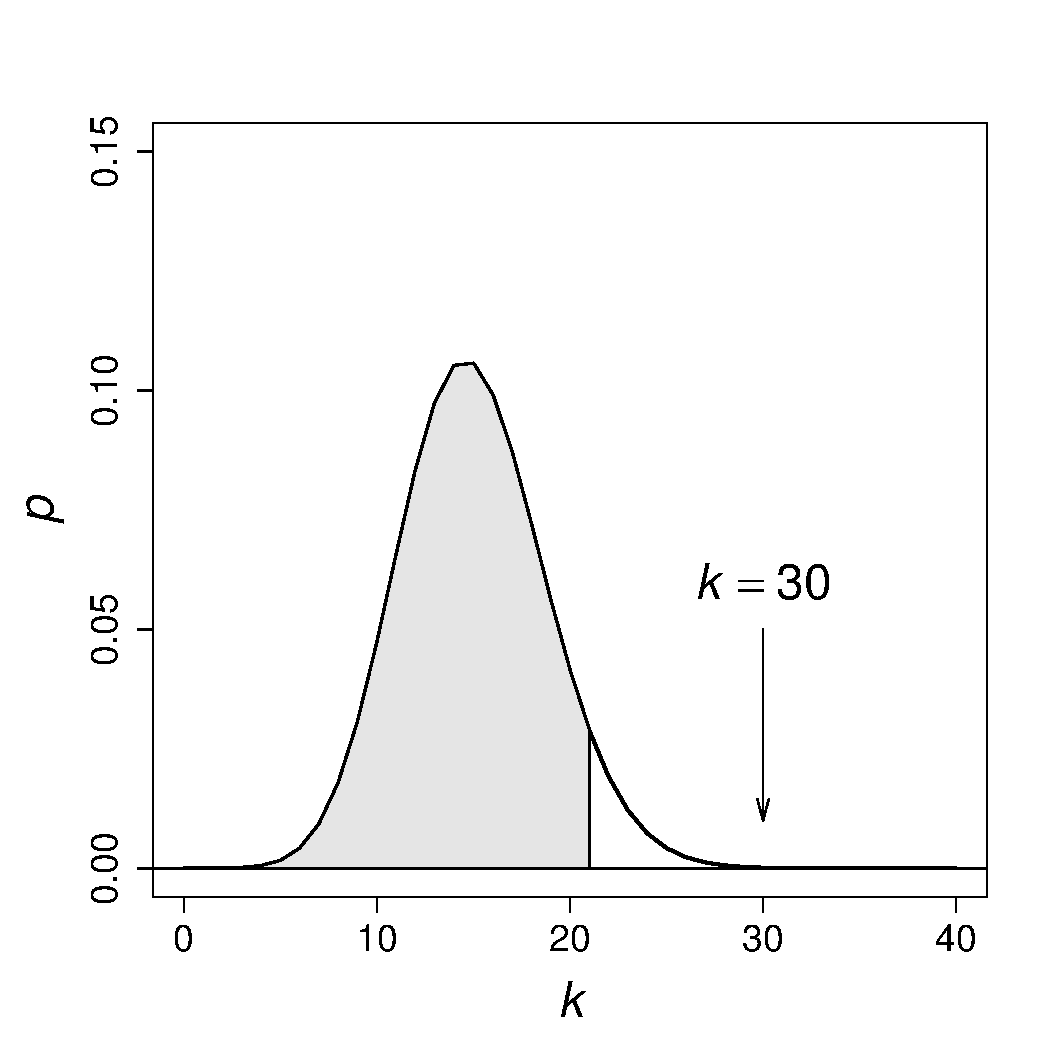
\includegraphics[width=0.6\textwidth]{../img/Gobinom.pdf}
\caption[Smoothed pmf for the Binomial Distribution]{\textbf{Smoothed pmf for the Binomial 
Distribution}.
   The smoothed variant of the probability mass
   function for the binomial distribution, with $p=0.06$ and
   $n=250$. Values for $k=0,1,\ldots,40$ are shown (the values for
   $k>40$ are nearly zero and are not shown). The observed value for
   $k$ of 30 lies outside of the range containing 95\% of the
   probability mass, and we reject the null hypothesis that the genes
   in the study set are not enriched in genes annotated by $t$. The
   $p$-value for this observation can be calculated by
   Equation~(\ref{eq:dbinomial}).}
   \label{fig:gobinom}
\end{figure}

\end{homeworkProblem}




\begin{homeworkProblem}{}
Calculate the probability of drawing
  20 blue balls from an urn containing 30 blue balls and 40 red balls
  if a total of 35 balls are drawn. Use the R command \texttt{choose(n,k)} to
  calculate $\binom{n}{k}$ and calculate the probability using
  Equation~(\ref{eq:hypergeometric}). Check your answer using the R
  command \texttt{dhyper(x,m,n,k)}, where $x$ is the number of blue
  balls drawn, $m$ is the total number of blue balls in the urn, $n$
  is the total number of red balls, and $k$ is the number of balls
  drawn from the urn.
  
  \begin{equation}
 \label{eq:hypergeometric}
p(k,n,p)  = \dfrac{\binom{m_t}{k}\binom{m-m_t}{n-k}}{\binom{m}{n}}.
\end{equation}


For full credit show your R code and the correct answer.
\end{homeworkProblem}


\begin{homeworkProblem}{}
 Consider the following R commands. The
  second line generates a matrix with 200 rows of 5 numbers each drawn
  at random from a normal distribution with mean 0 and standard
  deviation 1. The third line uses the R command \texttt{apply} to
  apply a \textit{t} test to each row (to test whether the mean value
  is significantly different from zero) and store the result in the
  vector P. The fourth line again uses \texttt{apply} to apply a Bonferroni
  correction to the $p$-values. 
\begin{verbatim}
N<-200
dat<-matrix(rnorm(5*N),nrow=N)
P<-apply(dat,1,function(x) t.test(x)$p.value)
P.corr <-apply(matrix(P),1,
      function(x,factor) min(1,x*factor),factor=N)
\end{verbatim}
  Now use the commands \texttt{sum(P$<=0.05$)} and
  \texttt{sum(P.corr$<=0.05$)} to count the number of entries for
  which the nominal $p$-values are significant and for which the
  corrected $P$-values are significant. Repeat the experiment with
  other values of $N$. Explain the results in light of the
  descriptions of the Bonferroni procedure.
  
  
  For full credit explain why multiple testing correction is needed in GO overrepresentation 
analysis. Explain how the Bonferroni correction works in 2-3 sentences. Explain your observations 
about the R code above.
\end{homeworkProblem}


\begin{homeworkProblem}{}
Use R to implement a function
  that calculates the probability according to the hypergeometric distribution of
  observing three genes annotated to $t$ ($n_t=3$) if $m_t=4$ genes in a
  population of $m=18$ genes are annotated to $t$ and the size of the study set
  is $n=5$. First implement an R function called \texttt{ch}
  (for \texttt{choose}, the binomial coefficient) using the builtin function
  \texttt{factorial}. Then implement a function \texttt{hypergeometric} using the
  function \texttt{ch}.

Check your answer from the
  previous problem using the built-in R function \texttt{dhyper}. Read
  the documentation for the function by entering \verb!>?dhyper! at
  the R prompt. 
  
  
  For full credit show the R code for both tasks and write the correct answer.
\end{homeworkProblem}



\begin{homeworkProblem}{}
 Now use the built-in R function
  \texttt{fisher.test} to calculate the probability with the Fisher
  exact test (which is identical to the above). In order to use this
  function, we have to construct a matrix representing the counts as a
  contingency table (consult the online R documentation for
  details). You may start with the following contingency table:

\begin{tabular}{|c|r|r|r|}
\hline
	& study ($n$) & not in study ($m-n$) & total ($m$)  \\
\hline
Annotated to $t$  & $a$ & $b$ & $m_t$   \\
\hline
Not annotated to $t$   & $c$ & $d$ & $m-m_t$  \\
\hline
          & $n$       &   $m-n$   & $m$ \\
\hline
\end{tabular}

First, consider what values $a$, $b$, $c$, and $d$ must have in terms
of $m,n,m_t$, and $n_t$. To calculate the $p$-value using the Fisher exact
test in R, enter the following command using the appropriate values
for $a$, $b$, $c$, and $d$.

\begin{lstlisting}[frame=single]
fisher.test(matrix(c(a,b,c,d),nrow=2),alternative="g")
\end{lstlisting}

The option \texttt{"alternative"} specifies the alternative hypothesis
for the statistical test. Since we are interested in
overrepresentation, the argument \texttt{"g"} for "greater" is
appropriate. 
Compare the results with the results of the previous exercise. Now
compare the $p$-value obtained for all possible different values of $k$.


For full credit show your R code.
\end{homeworkProblem}

\begin{homeworkProblem}{}
 An equivalent result can be
  obtained using the function \texttt{phypergeom}. Note that
  \texttt{lower.tail=F} implies that the function will take the sum
  over the upper tail, i.e., $X > x$, but that the definition of the
  Fisher's exact test implies $X\geq x$. Using the quantities for
  $n_t$, $m_t$, $m$, and $n$ from the previous exercise, check that
  you get the same result with the following command. Read the R
  documentation if anything is unclear.

\begin{lstlisting}[frame=single]
phyper(n.t - 1,m.t,m-m.t,n,lower.tail=F)
\end{lstlisting}
For full credit show your R code.
\end{homeworkProblem}



\begin{homeworkProblem}
In the description of the MGSA algorithm given in the previous
section, the values of the parameters $\alpha, \beta$, and $p$ were
taken as givens. However, these values are not known in
advance. Although it is possible to estimate them by running MGSA with
many different combinations of values for $\alpha, \beta$, and $p$,
the estimation of the parameters $\alpha$, $\beta$, and $p$ can also be
easily integrated directly into the MCMC algorithm. The parameters now
must be explicitly considered in the joint probability distribution:
\begin{equation*}
  P(p,T,H,\alpha,\beta,O) =  P(p)P(T|p)P(H|T)P(\alpha)P(\beta)P(O|H,\alpha,\beta),
\end{equation*}

Consult the original publication of MGSA (Bauer S, Gagneur J, Robinson PN. GOing Bayesian: 
model-based gene set analysis of genome-scale data. Nucleic Acids Res. 2010;38:3523-32), and 
explain this algorithm in your own words.

\end{homeworkProblem}



\begin{homeworkProblem}{}
Download the Yeast dataset that
  was analyzed for the original publication of the MGSA
  method.\footnote{%
    Available at
    \texttt{http://nar.oxfordjournals.org/content/38/11/3523} or
    alternatively at the PubMed website under the PubMed ID
    20172960; the article is freely available.} The
  dataset can be downloaded as part of the Supplementary Data for the
  article (the second file is the study set, and the third file is the
  population set). Now compare the results of the term-for-term and
  parent-child union\footnote{Grossmann S, Bauer S, Robinson PN, Vingron M. Improved detection of
overrepresentation of Gene-Ontology annotations with parent child analysis.
Bioinformatics. 2007 Nov 15;23(22):3024-31} with the results
  of MGSA. Perform the analysis with the Ontologizer. Now read the
  discussion in the original publication of MGSA. Do you agree with
  the comments \textit{of trees and forests}?

\end{homeworkProblem}



% %----------------------------------------------------------------------------------------
% \cleardoublepage\include{FrontBackMatter/Bibliography} % Bibliography
\end{document}